\chapter{Introduction}\label{C:intro}
Modern enterprises need to respond effectively and quickly to opportunities in today's competitive and global
markets. To accommodate business agility, companies are supposed to utilise existing business processes while
exposing the various packaged applications found spread throughout the enterprise in a highly standardized manner. A contemporary approach for addressing these critical issues is embodied by (Web) services that can be 
easily assembled to form a collection of autonomous and loosely coupled business processes \cite{Papazoglou}.

The emergence of Web services developments and standards in support of automated business integration has 
driven major technological advances in the integration software space, most notably, 
the service oriented archiecture (SOA) \cite{Dan:2008}. In an SOA, software resources are packaged as 
Web services, which are well defined, self-contained modules that provide standard business functionality
and are independent of the state or context of other services \cite{Ran}.

A Web service is a software system allowing to expose services via the Internet. The 
SOA promotes the composition of coarse-grained Web services to build more complex
Web applications using standards such as WS-BPEL \cite{std/ws-bpel2}. Because of the convenience, low cost \cite{Aboolian} and capacity to be composed into high-level business processes, Web service technology is becoming increasing popular.

%Web services are hosted in heterogeneous server clusters or co-location centers 
%that were widely distributed across different network providers and 
%geographic regions. In recent years,
%Web services are increasingly being deployed in clouds such as Amazon EC2, Windows Azure, and Rackspace. According to a popular web traffic analyzer Alexa\cite{He}, 4\% of Alexa`s top
%1 million use EC2/Azure and 96\% Web services were hosted in other platforms.

With the ever increasing number of functional similar Web services being available on the Internet, the Web service providers (WSPs) are trying to improve the quality of service (QoS) to become competitive in the market.  
QoS, also known as non-functional requirements to  Web services, is the degree to which a service meets specified requirements or user needs \cite{4061431}, such as response time, security and availability. 
Among numerous QoS measurements, service response time is a critical factor for many real-time services, e.g. traffic service or finance service. 
Service response time has two components: transmission time (variable with message size) and network latency \cite{Johansson}. 

%\begin{figure}[h!]
	%\centering
		%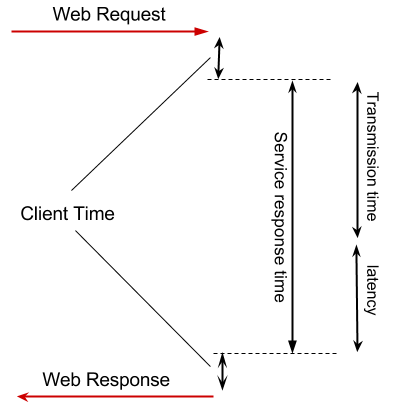
\includegraphics[width=0.3\textwidth]{pics/latency.png}
	%\caption{Service response time}
%\end{figure}

Study \cite{916684} shows that network latency is a significant component of service response delay.
Ignoring network latency will underestimate response time by more than 80 percent \cite{Sun}, since network latency is related to network topology as well as physical distance \cite{distanceMetrics}. 
To reduce the network latency, WSPs need to allocate Web services to a user concentrated area so that the overall network latency is minimized. 

According to a popular Web traffic analyzer, Alexa, 96\% of top 1 million Web services were hosted
in heterogeneous server clusters or co-location centers \cite{He} that were widely distributed across different network
providers and geographic regions. Hence, it is not only necessary but also urgent to provide an effective Web services allocation guide to WSPs so that they can be benefited.

Ideally, WSPs could deploy their services to each user center in order to provide the best quality.
However, the more services deployed, the better the quality and the higher cost. 



The main goal of Web service location-allocation is providing a Web service allocation plan to WSPs so that it minimizes
the cost as well as optimizes quality of services.


\section{Objectives}
%The aim of this project is to propose a model for the Web service location-allocation problem so that it can be tackled by Evolutionary Multi-objective Optimization (EMO). 
%Furthermore, based on this model, develop a Multi-objective PSO based approach to solve the Web service location-allocation problem. 
The aim of this project is to propose a multi-objective PSO based approach to produce 
a set of near optimal solutions of Web service location-allocation, so that cost and 
overall network latency are close to minimum. Then, the WSPs could use the algorithm 
which proposed by this paper, to select an optimal plan based on their funds. The main
objectives are:

\begin{enumerate}
	\item To model the Web service location-allocation problem so that it can be tackled
		by Evolutionary Multi-objective Optimization (EMO).
	\item To develop a Multi-objective PSO based approach to the Web service location-allocation problem.
\end{enumerate}




\section{Achievements to Date}
In the first trimester, we have accomplished the two objectives. We modelled the service location-allocation problem with a set of matrices as input and a matrix as output. 
Based on this model, we further developed a multi-objective Particle Swarm Optimization (PSO) based algorithm to solve this problem. 

We have conducted a series of experiement that runs on four test cases. The experimental results were fully analyzed by compared between different parameter settings and 
compared with a NSGA-II based approach.
The experiments show that the PSO-based algorithm performed significantly better than NSGA-II based approach in terms of both effectiveness and efficiency. The experiments also show
a critical parameter: transfermation threshold, plays an important role in determining the solutions. 

\section{Future Work}
We have done the first objective of the project. The second objective is not fully 
finished for the following reasons: 1.The impact of parameter settings was not fully studied. 2. The effectiveness was not fully verified. 

Therefore, in the second half of the project, we mainly focus on: Further improved the algorithm based on analyze the parameter settings. Develop a single-objective based PSO and compare the result of it with the result of multi-objective based PSO.
%During the study we discovered that there is no common model that generally fits all multi-objective 
%optimization algorithms. 
%Although most Evolutionary Multiobjective Optimization (EMO) algorithms share similar representation, there are
%many subtle differences that prevent them from sharing a general model. Genetic algorithm (GA) uses a 
%string-liked representation (e.g., matrix $A'$) that naturally good at solving discrete problem (e.g., binary problem). 
%However, in PSO, particles are ``moving'' in a continuous hyperplane. 
%Therefore, the representation of particle (e.g., matrix $A$) is continuous.

%\parbox{.45\linewidth}{
%{\centering
%$
%A = \bbordermatrix{~ & j_{1} & j_{2} & j_{3}\cr
				%s_{1}	&0.12 &0.87 &0.42	\cr
				%s_{2}	&0.07  &0.32 &0.95	\cr
				%s_{3}	&0.76 &0.64 &0.27	\cr}
%$
%\\}
%}
%\parbox{.45\linewidth}{
%{\centering
%$
%A' = \bbordermatrix{~ & j_{1} & j_{2} & j_{3}\cr
					%s_{1}	&0 &1 &0	\cr
					%s_{2}	&0  &0 &1	\cr
					%s_{3}	&1 &1 &0	\cr}
%$
%\\}
%}

%In order to cope with the subtle differences between two algorithms, we employed a transfermation 
%technique with a parameter: threshold.

%\begin{equation}
	%x_{id} = 
	%\begin{cases}
		%1 & \quad \text{if } x_{id} > threshold \\
		%0 & \quad \text{otherwise} \\
	%\end{cases}
%\end{equation}

%This transfermation is applied on each variable of a particle before evaluation, 
%transform from continuous representation $A$ to
%$A'$. As a result, the fitness functions could be applied on 
%PSO-based algorithm as well as genetic algorithm-based algorithm.

%However, it completely changed the explanation of the original representation.

%In the originl design, $A'$ represents a particle or chromosome which denotes a solution or 
%service deployment plan where $a_{sj}$ is a binary value 1 or 0 to indicate whether 
%a service $s_i$ is allocate to a location $j_i$ or not. 
%In continuous representation $A$, each entry represents a probability of service $s_i$ \testbf{NOT} allocate in a location $j_i$. 
%We could manipulate the solutions by adjusting the threshold. For example, the solution is different by applying 
%different threshold values.

%We employed this approach and the experimental results show that the threshold profoundly affect the final solution set. Therefore, it leads to a new problem, how to choose an appropriate threshold.

%So far, we considered two approaches. First, based on current model, developing a dynamic threshold which automated adjust its value along with the iteration. Second, 
%developed a binary PSO based algorithm which could directly applied the binary-matrix representation.



%\section{The Problem}
%The Web service location-allocation problem is essentially a multi-objective optimization problem \cite{Multiobjective}, for which there are two conflict objectives,
%to provide optimal QoS to Web service users and to consume minimal deployment cost.
%This problem can be classified as a multidimensional knapsack problem (MKP), therefore, it is
%considered NP-hard due to the fact that the combinatorial explosion of the search space 
%\cite{Vanrompay}.


%Very few researches have studied the service location-allocation problem and most of the researchers treat this problem as a single objective problem.
%\cite{Aboolian} \cite{Sun} try to solve the problem by using integer linear programming techniques.
%In particular, \cite{Sun} solved this problem by employing greedy and linear relaxations of Integer transpotation problem.
%However, integer programming (IP) is very effective for small-scale or mid-scale 
%MKP but suffers from large memory requirement for large-scale MKP \cite{Hwang11aninteger}.

%So far, to the best of our knowledge, there is few research has considered using Evolutionary Computation (EC)
%techniques to solve the location-allocation problem. 



%Therefore, in this paper we first developed a model for
%location-allocation problem so that it can be tackled by EC algorithms. Secondly, we employed Binary Particle
%Swarm Optimization algorithm (BPSO) to solve this problem. Thirdly, we expand the location-allocation problem
%as a multi-objective problem. A multi-objective model is developed for further improvement. The
%the service location-allocation problem as a multi-objective problem.Therefore, in this paper we will treat service location-allocation problem as a multi-objective problem. 

%Evolutionary multi-objective optimization (EMO) methodologies
 %is ideal for solving multi-objective optimization problems \cite{key:article}, since EMO works with a population of solutions and 
%a simple EMO can be extended to maintain a diverse set of solutions.
%With an emphasis for moving toward the true Pareto-optimal region, an EMO can be used to find multiple Pareto-optimal solutions in 
%one single simulation run \cite{OptimizationElectrical}. 
%The first major challenge is to model the Web service location-allocation into a suitable representation
%so that the EC algorithms and EMO techniques can be employed. The second challenge is develped a binary PSO
%based and a multi-objective PSO based algorithm to solve this problem.
%Among numerous EMO algorithms,
%Non-dominated sorting GA (NSGA-II) \cite{996017}, Strength Pareto Evolutionary Algorithm 2 (SPEA-2) \cite{Deb} have become standard approaches. 
%Some schemes based on particle swarm optimization (PSO) approaches are also proposed \cite{Elhossini} \cite{Huang}.
%NSGA-II is one of the most widely used methods for generating the Pareto frontier, because it can keep diversity without specifying any additional parameters \cite{Deb06referencepoint}.
%In this paper, we propose to use NSGA-II to solve the Web service location-allocation problem, which has two objectives, to minimize
%cost and deployment network latency.

%Several multiobjective optimization algorithms are based on Particle Swarm Optimization such as Multi-objective Particle Swarm Optimization (MOPSO) \cite{1304847}, Nondominated Sorting 
%Particle Swarm Optimization (NSPSO) \cite{NSPSO}. The performance of different multi-objective algorithms was compared in \cite{1304847} using
%five test functions. These algorithms are NSGA-II, PAES \cite{781913}, Micro-GA \cite{Micro} and MOPSO. The results show that MOPSO was able to generate the best set of nondominated solutions
%close to the true Pareto front in all test functions except in one function where NSGA-II is superior.

%Raquel and et al. \cite{Raquel} proposed a multi-objective Particle Swarm Optimization with crowding distance (MOPSOCD) that extends the MOPSO. The mechanism of crowding distance is 
%incorporated into the algorithm specifically on global best selection and in the delection method of an external archive of nondominated solutions. The diversity of nondominated
%solutions in the external archive is amintained by using the mechanism of crowding distance together with a mutation operator. The performance shows that MOPSOCD is highly 
%competitive in converging towards the Pareto front and has generated a well-distributed set of nondominated solutions.


%In this paper, we proposed to use multi-objective to solve the Web service location-allocation problem, which has two objectives, to minimize cost and deployment network latency.
%We consider the problem faced by a WSP who has existing facilities but wishes to use the collected data to re-allocate their services in order to maximum their profit.
%The WSP must decide on facility locations from a finite set of possible locations. 
%In order to make a decision, the WSP must first analyze the data collected from current use of services. 
%The collected data should include the records of invocations from each unique IP address.
%Therefore, based on these data, the WSP could summarize several customer demands concentrated on \textit{n} discrete nodes \cite{Aboolian}, namely user centers. 
%We assume that the WSP has already done this step and a list of user centers and candidate service deployment locations are given.
%In addition to deciding locations to of the services, information about network latency between user centers and candidate locations is needed. 
%Exist datasets in \cite{6076756} \cite{5552800} contain latency information collected from the real world. 
%\section{Objectives}
%The aim of this project is to propose two models for service location-allocation problem so that it 
%can be tackled by single-objective and multi-objective evolutionary computation algorithms. 
%Furthermore, we develped a binary PSO based and a multi-objective based approaches to solve the problem. 
%The multi-objective PSO based approach to produce a set of near optimal solutions of service 
%location-allocation, so that cost and overall network latency are close to minimum. Then, the 
%service provider could use the algorithm which proposed by this paper, to select an optimal 
%plan based on their funds. 
%The main objectives can be divided into three categories:
%\begin{itemize}
	%\item Developed two model for the Web service location-allocation problem so that it can be tackled by binary PSO and multi-objective PSO.
	%\item To develop a binary PSO and a multi-objective PSO based approach to the Web service location-allocation problem.
	%\item To evaluate our proposed approach using some existing datasets.
%\end{itemize}

%\section{Major Contribution}
%The project has three major contribution. Firstly, a new model for the Web service location-allocation is
%developed, which utilises matrix representation so that it can be easily tackled by any evolutionary Algorithms
%such as GA and PSO. The second contribution is to developed a binary PSO \cite{} so solve the 
%location-allocation problem. The last contribution is to further improve the 
%quality of location-allocation plan by 
%\section{Organisation}
%In Section \ref{sec:Background} we introduce the background of multi-objective PSO and NSGA-II.
%In Section \ref{sec:problem} we provide models of the service location allocation problems. Section \ref{sec:algorithm_des} develops a MOPSOCD based algorithm. 
%The experimental design and results evaluation are shown in Section \ref{sec:experiment}. Section \ref{sec:conclusion} provides a brief summary.

\chapter{Background Survey}
\section{Single-objective methods}
Very few researches have studied the Web service location-allocation problem and most of the researchers treat this problem as a single objective problem.
\cite{Aboolian} \cite{Sun} try to solve the problem by using integer linear programming techniques.
In particular, \cite{Sun} solved this problem by employing greedy and linear relaxations of Integer 
transpotation problem. However, the major problem for this approach is that linear programming is not scaling.

Huang \cite{EnhancedGenetic} proposed an enhanced genetic algorithm (GA)-based approach, which make use of the integer scalarization technique to solve this problem.
GA \cite{man1996genetic} is an Evolutionary algorithm (EA) that uses genetic operators to obtain optimal solutions without any assumptions about the search space.
This algorithm solves the problem with one objective and one constraint. However there are some deficiencies in the
integer scalarization techniques \cite{Multiobjective}. Firstly, decision makers need to choose appropriate weights for the objectives to retrieve a satisfactorily solution. 
Secondly, non-convex parts of the Pareto set cannot be reached by minimizing convex combinations of the object functions.



\section{Multi-objective methods}
So, far, to the best of our knowledge, there is no other researcher has considered the Web service location-allocation problem as a multi-objective problem. 
In previous research, we proposed a NSGA-II \cite{996017} based approach to Web service location-allocation problem. 
NSGA-II is a multi-objective algorithm based on GA. It is one of the most widely used methods for generating the Pareto frontier, 
because it can keep diversity without specifying any additional parameters \cite{Deb06referencepoint}.
When it is used for problems with only two objectives, NSGA-II performs relatively well in both convergence and  computing speed. However, NSGA-II has been
criticized for its high computational cost and bad performance on applications with more than two objectives \cite{nsga2_cri}.

NSGA-II permits a remarkable level of flexibility with regard to performance assessment and design
specification. NSGA-II assumes that every chromosome in the population has two attributes: a non-domination rank in the population and a local crowding
distance in the population. The goal of NSGA-II is to converge to the Pareto front as possible and with even spread of the solutions on the front by controlling
the two attributes. The algorithm starts with a random initialization population. Once the population is sorted based on non-domination sorting, a rank is assigned to each
chromosome. Then, a parameter called crowding distance is calculated for each individual. The crowding distance is a measure of how close an individual is to
its neighbors. A large average crowding distance will result in better diversity in the population.
Parents are selected from the population by using tournament selection based on the rank and the crowding distance. An individual is selected in the rank if it
is smaller than the other or if the crowding distance is greater than the other. The population with the current population and current offsprings is sorted
again based on non-domination and only the best $N$ individuals are selected,
where $N$ is the population size. The selection is based on rank and the on crowding distance on the last front.

Several multiobjective optimization algorithms are based on Particle Swarm Optimization such as Multi-objective Particle Swarm Optimization (MOPSO) \cite{1304847}, Nondominated Sorting 
Particle Swarm Optimization (NSPSO) \cite{NSPSO}. The performance of different multi-objective algorithms was compared in \cite{1304847} using
five test functions. These algorithms are NSGA-II, PAES \cite{781913}, Micro-GA \cite{Micro} and MOPSO. The results show that MOPSO was able to generate 
the best set of nondominated solutions close to the true Pareto front in all test functions except in one function where NSGA-II is superior.

Raquel and et al. \cite{Raquel} proposed a multi-objective Particle Swarm Optimization with crowding distance (MOPSOCD) that extends the MOPSO. The mechanism of crowding distance is 
incorporated into the algorithm specifically on global best selection and in the delection method of an external archive of nondominated solutions. The diversity of nondominated
solutions in the external archive is amintained by using the mechanism of crowding distance together with a mutation operator. The performance shows that MOPSOCD is highly 
competitive in converging towards the Pareto front and has generated a well-distributed set of nondominated solutions. Another major advantage for PSO-based algorithms is low
computation cost. It is much effective than other EC algorithms.

\section{Summary}
Previous researchers have studied Web services location-allocation problem with
single-objective algorithms. These approaches have many disadvantages in comparison with
multi-objective algorithms. In particular, Evolutionary Multi-objective Optimization 
algorithms such as NSGA-II and Multi-objective PSO based algorithms show advantages in 
terms of quality of solution and computational time.


%NSGA-II was the first Evolutionary Multi-objective 
%algorithm that applied to this problem.

%\section{Particle Swarm Optimization (PSO)}
%PSO proposed by Kennedy and Eberhart in 1995 \cite{488968}. Similar to evolutionary algorithms (EA), PSO is a population based technique inspired by the swarm behavior of birds and fishes during their search for food. PSO is a meta heuristic in which each individual, called a particle, flies in its own direction and velocity searching for a good solution in the search space. The underlying phenomenon of PSO is optimized by social interaction in the population where all particles communicate their information to direct their movement.


%PSO is based on the principle that each solution can be represented as a 
%particle in the swarm. Each particle has a random initial position in the 
%search space which is represented by a vector $x_i = (x_{i1}, x_{i2}, \dots, x_{iD})$, where \emph{D} is the dimensionality of the search space. Particles move in the 
%search space to search for the optimal solutions. Each particle has a velocity, 
%represented as $v_i = (v_{i1}, v_{i2}, \dots, v_{iD})$ which is limited by a 
%predefined maximum velocity, $v_{max}$ and  $v_{id}$ $\in$ $[-v_{max}, v_{max}]$. 
%During the search process, each particle maintains a record of position its 
%previous best performance, called pbest. The best position of its neighbours 
%is also recorded, which is gbest. The position and velocity of each particle are 
%updated according to the following equations:

%\begin{equation}
	%x^{t+1}_{id} = x^{t}_{id} + v^{t+1}_{id}
%\end{equation}
%\begin{equation}
	%v^{t+1}_{id} = w * v^{t}_{id} + c_1 * r_{1i} * (p_{id} - x^t_{id}) + c_2 * r_{2i} * (p_{pg} - x^t_{id})
%\end{equation}

%In the two equations, $t$ shows the $t^{th}$ iteration. \emph{d} $\in$ \emph{D} 
%shows the 
%$d^{th}$ dimension. \emph{w} is the inertia weight used to balance the local search and 
%global search abilities of PSO. $c_1$ and $c_2$ are acceleration constants. 
%$r_{1i}$ and $r_{2i}$ are random constants uniformly distributed in $[0, 1]$. $p_{id}$ and $p_{gd}$ denote the values of pbest and gbest in $d^{th}$ dimension.

%\section{Binary PSO}
%PSO was originally developed to address continuous optimisation problems. 
%Therefore, the representation for both position and velocity of a particle in 
%PSO is a vector of real numbers. However, this representation is not suitable 
%for many discrete optimisation problems. To address the discrete problem, in 1997 
%Kennedy and Eberhart developed a binary 
%particle swarm optimisation (BPSO) \cite{637339}.
%In BPSO, the position of each particle is a vector of binary numbers, which are 
%restricted to 1 or 0.  The velocity in BPSO represents the probability of the 
%corresponding position taking value of 1. To transfer the velocity value between 
%0 and 1, we used a sigmoid function to achieve this. The following equation is 
%used to update the position of each particle:

%\begin{equation}
		%f(n) = 
		%\begin{cases}
			%1 & \quad \text{if } rand() < s(v_{id})\\
			%0 & \quad \text{otherwise} \\
		%\end{cases}
%\end{equation}
%\begin{equation}
	%s(v_{id}) = \frac{1}{1 + e^{-v_{id}}}
%\end{equation}
%The rand() is a random number selected from a uniform distribution in $(0, 1)$.




%\section{Evolutionary Computation}

%\subsection{Genetic Algorithms (GAs)}
%GA \cite{man1996genetic} is a powerful tool to solve combinatorial optimization problems. It is an iterative procedure based on a constant-size population. In a GA, a population of strings (called chromosomes
%or the genotype of the genome), which are encoded as candidate solutions (called individuals, creatures, or phenotypes) to an optimization problem, evolves towards better solutions. 
%Each genome is associated with a fitness value based on a fitness function that indicates how close it comes to meeting the overall specification, when compared to other genomes in the
%population. The fitness value of an individual is also an indication of its chances of survival and reproduction in the next generation. A typical genetic algorithm requires a genetic
%representation of the solution domain and a fitness function to evaluate the solution domain. Since a chromosome from the population represents a solution, when the algorithm starts, 
%the whole population moves like one group towards an optimal area so the GA searches from a population of solutions rather than a single solution. Integer scalarization technique \cite{Multiobjective} is 
%used to solve multi-objective problems with GA. It predefines a weight for each objective.
%\subsection{Nondominated Sorting Genetic Algorithm II (NSGA-II)}
%NSGA-II is a multi-objective algorithm based on genetic algorithm (GA) \cite{man1996genetic}. When used for problems with only two objectives, NSGA-II performs 
%relatively well in both convergence and  computing speed. It permits a remarkable level of flexibility with regard to 
%performance assessment and design specification. NSGA-II assumes that every chromosome in the population has two 
%attributes: a non-domination rank in the population and a local crowding distance in the population. The goal of 
%NSGA-II is to converge to the Pareto front as possible and with even spread of the solutions on the front by 
%controlling the two attributes. 

%The algorithm starts with a random initialization population. Once the population is sorted based on non-domination sorting, a rank is assigned to each chromosome.
%Then, a parameter called crowding distance is calculated for each individual. The crowding distance is a measure of how close an individual is to its neighbors. A large 
%average crowding distance will result in better diversity in the population. 

%Parents are selected from the population by using tournament selection based on the rank and the crowding distance. An individual is selected in the rank if it is smaller than the other or 
%if the crowding distance is greater than the other. The selected population generates offsprings using crossover and mutation operators. 

%The population with the current population and current offsprings is sorted again based on non-domination and only the best N individuals are selected, where N is the population size.
%The selection is based on rank and the on crowding distance on the last front.

%\subsection{Summary}
